\section{Часть III: Разделения}

\begin{frame}
    \centering
    \usebeamerfont{title}\insertsectionhead

    \vspace{0.5cm}
    
\includegraphics[scale = 0.2]{pics/utia-money.png}
\end{frame}

\begin{frame}{Мон. формулы vs. мон. схемы}

    \begin{minipage}{0.5 \textwidth}
        \centering
        \textbf{Нижняя оценка}
    \end{minipage}%
    \begin{minipage}{0.5 \textwidth}
        \centering
        \textbf{Верхняя оценка}
    \end{minipage}
    
    \begin{center}
        $\varphi$ формула маленькой ширины
	\end{center}


    \pause
    \vspace{0.4cm}

    \begin{minipage}{0.5 \textwidth}
        \centering
        резолюционная глубина
    \end{minipage}%
    \begin{minipage}{0.5 \textwidth}
        \centering
        резолюционная ширина
    \end{minipage}

    \pause
    \vspace{0.3cm}
    \begin{center}
        $\Downarrow$
        
        \vspace{0.3cm}
        $\Search_{\varphi \circ \Ind}$
    \end{center}
 
    \pause
    \vspace{0.3cm}
    \begin{minipage}{0.5 \textwidth}
        \centering
        $\Downarrow$ [GPW 16]

        \vspace{0.3cm}

        нижняя оценка на формулы
    \end{minipage}%
    \begin{minipage}{0.5 \textwidth}
        \centering
        $\Downarrow$

        \vspace{0.3cm}

        верхняя оценка на схемы
    \end{minipage}


    \pause
    \vspace{1cm}
    Цель найти такую формулу маленькой ширины, что:
    \begin{itemize}
        \item res-depth $n^{\varepsilon}$;
        \item res-width $\bigO{1}$.
    \end{itemize}
\end{frame}


\begin{frame}{Pebbing}

    \begin{center}
        \tikzstyle{vert} = [
    circle,
    draw,
    inner sep = 0pt,
    minimum size = 0.45cm,
    fill = LEIorange!5
]
\tikzstyle{pstyle} = [alt = <{#1}>{fill = LEIorange!50}{}]
    
\tikzset{
    xcenter around/.style 2 args = {
        execute at end picture = {%
            \useasboundingbox let \p0 = (current bounding box.south west),
            \p1 = (current bounding box.north east),
            \p2 = (#1),
            \p3 = (#2) in ({min(\x2 + \x3 - \x1, \x0)}, \y0) rectangle ({max(\x3 + \x2 - \x0, \x1)},\y1);
        }
    }
}

\begin{tikzpicture}[xcenter around = {-2.1, -2.1}{2.1, 0.1}]
    \node at (3.6, -0.6) {
\includegraphics[scale = 0.09]{pics/utia-rest.png}};
    
    \node[vert, pstyle = 2, pstyle = {9-}, alt = <10>{fill = red!60}{}] (a) at (0, 0) {$r$};
    \node[vert, pstyle = 4, pstyle = {7-}] (b) at (-1, -1) {$x$};
    \node[vert, pstyle = {8-}] (c) at (1, -1) {$y$};
    \node[vert, pstyle = {3-4}, pstyle = {6-}] (d) at (-2, -2) {$z$};
    \node[vert, pstyle = {3-4}, pstyle = {6-}] (e) at (0, -2) {$u$};
    \node[vert, pstyle = 3, pstyle = {8-}] (f) at (2, -2) {$w$};

    \draw[->] (b) -- (a);
    \draw[->] (c) -- (a);
    \draw[->] (d) -- (b);
    \draw[->] (e) -- (b);
    \draw[->] (e) -- (c);
    \draw[->] (f) -- (c);
\end{tikzpicture}        
    \end{center}

    \pause
    \begin{itemize}
        \item $(\neg r)$;
            \pause
        \item $(z), (u), (w)$;
            \pause
        \item $(\neg z \lor \neg u \lor x)$.    
    \end{itemize}

    \pause
    \begin{lemma}
        Для этой формулы:
        \begin{itemize}
            \item res-depth $\approx \sqrt{n}$;
            \item res-width $\bigO{1}$.
        \end{itemize}
    \end{lemma}

    \pause
    Степень в $\NS$ тоже $\approx \sqrt{n}$. $\Rightarrow$ Разделение мон. Span Programs и мон. схем.
\end{frame}


\begin{frame}{Монотонные Span Programs над полем $\field$ [Karchmer, Wigderson 93]}

    \only<1>{
        \begin{center}
            \begin{tabular}{|c|cccccccc|}
                \hline
                $x_1$ & 0 & 2 & 3 & 1 & 0 & 2 & 1 & 0\\
                $x_3$ & 2 & 1 & 0 & 0 & 2 & 0 & 0 & 1\\
                $x_4$ & 1 & 0 & 0 & 0 & 0 & 0 & 0 & 0\\
                $x_5$ & 3 & 2 & 1 & 4 & 0 & 2 & 1 & 0\\
                $x_1$ & 0 & 2 & 3 & 1 & 3 & 2 & 4 & 0\\
                \hline
            \end{tabular}
        \end{center}
    }
      
	\only<2->{
        \begin{minipage}{0.5\linewidth}
            \def\firstrow{
            	$x_1$ & 1 & 0 & 1\\
                $x_1$ & 1 & 1 & 0\\
            }
            \only<5-6>{
                \def\firstrow{
            	    \rowcolor{green!40}[1.001\tabcolsep][1.001\tabcolsep] $x_1$ & 1 & 0 & 1\\
                    \rowcolor{green!40}[1.001\tabcolsep][1.001\tabcolsep] $x_1$ & 1 & 1 & 0\\
                }
            }

            \def\secondrow{
                $x_2$ & 0 & 1 & 1 \\
                $x_2$ & 1 & 1 & 0 \\
            }
            \only<8-9>{
                \def\secondrow{
            	    \rowcolor{red!40}[1.001\tabcolsep][1.001\tabcolsep] $x_2$ & 0 & 1 & 1 \\
                    \rowcolor{red!40}[1.001\tabcolsep][1.001\tabcolsep] $x_2$ & 1 & 1 & 0 \\
                }
            }

            \def\thirdrow{
                $x_3$ & 0 & 1 & 1 \\
                $x_3$ & 1 & 0 & 1 \\
            }
            \only<5-6>{
                \def\thirdrow{
            	    \rowcolor{green!40}[1.001\tabcolsep][1.001\tabcolsep] $x_3$ & 0 & 1 & 1 \\
                    \rowcolor{green!40}[1.001\tabcolsep][1.001\tabcolsep] $x_3$ & 1 & 0 & 1 \\
                }
            }
              
            \begin{center}
                \begin{tabular}{|c|ccc|}
                    \hline
                    \firstrow
                    \secondrow
                    \thirdrow
                    \hline
                \end{tabular}
            \end{center}
        \end{minipage}%
        \begin{minipage}{0.5\linewidth}
            \pause
            \pause
            \begin{itemize}
                \item Верно ли, что $(1, 1, 1, \dots)$ в линейной оболочке выбранных векторов?
                \pause  
                \item $f(1, 0, 1) = \only<4-5>{~?} \only<6->{1;}$
                \pause
                \pause
                \pause
                \item $f(0, 1, 0) = \only<7-8>{~?} \only<9->{0;}$
                \pause
                \pause
                \pause
                \item $\Maj(x_1, x_2, x_3)$.
            \end{itemize}
        \end{minipage}
    }
    
    \vspace{0.15cm}

    \pause
    Размер~--- число столбцов.

    \pause
    \vspace{0.3cm}

    \begin{minipage}{0.5\linewidth}
        \begin{center}
        	$\AND$
            \vspace{0.05cm}
            
            \begin{tabular}{|c|cc|}
                \hline
                $x_1$ & 1 & 0\\
                $x_2$ & 0 & 1\\
                \hline
            \end{tabular}
        \end{center}
    \end{minipage}%
    \begin{minipage}{0.5\linewidth}
        \begin{center}
        	$\OR$
            \vspace{0.05cm}
            
            \begin{tabular}{|c|c|}
                \hline
                $x_1$ & 1\\
                $x_2$ & 1\\
                \hline
            \end{tabular}
        \end{center}
    \end{minipage}

    \pause
    \begin{lemma}[Pudl{\'{a}}k, Sgall 98]
        Монотонные Span Programs моделируют монотонные формулы.
    \end{lemma}
\end{frame}

\begin{frame}{Span Programs и Nullstellensatz}

    \begin{lemma}[Модификация Pudl{\'{a}}k, Sgall 98]
        $\NS$-доказательство $\varphi \circ g$ степени $d$ $\Rightarrow$ MSP для $F_{\varphi \circ g}$
        размера $n^d$.
    \end{lemma}

    \pause
    \begin{itemize}
        \item $\sum h_i(z) f_i(z) = 1$;
        \item $\Ind_m(x, y) = \sum\limits_{s \in [m]} \mathds{1}_{x = s} \cdot y_s$;
        \item $\sum h_i(\Ind(x, y)) f_i(\Ind(x, y)) = 1$.
    \end{itemize}

    \pause
    \vspace{0.7cm}
    \begin{center}
        Неплохо бы разделить $\NS$ степень и резолюционную ширину.        
    \end{center}
\end{frame}

\begin{frame}{MSP vs. мон. схемы}

    \begin{minipage}{0.5 \textwidth}
        \centering
        \textbf{Нижняя оценка}
    \end{minipage}%
    \begin{minipage}{0.5 \textwidth}
        \centering
        \textbf{Верхняя оценка}
    \end{minipage}
    
    \begin{center}
        $\varphi$ формула маленькой ширины
	\end{center}


    \vspace{0.4cm}

    \begin{minipage}{0.5 \textwidth}
        \centering
        резолюционная ширина
    \end{minipage}%
    \begin{minipage}{0.5 \textwidth}
        \centering
        $\NS$ степень
    \end{minipage}

    \vspace{0.3cm}
    \begin{center}
        $\Downarrow$
        
        \vspace{0.3cm}
        $\Search_{\varphi \circ \Ind}$
    \end{center}
 
    \vspace{0.3cm}
    \begin{minipage}{0.5 \textwidth}
        \centering
        $\Downarrow$ [GPW 16]

        \vspace{0.3cm}

        нижняя оценка на мон. схемы
    \end{minipage}%
    \begin{minipage}{0.5 \textwidth}
        \centering
        $\Downarrow$ [PS 98]

        \vspace{0.3cm}

        верхняя оценка на MSP
    \end{minipage}


    \vspace{1cm}
    Цель найти такую формулу маленькой ширины, что:
    \begin{itemize}
        \item res-width $n^{\varepsilon}$;
        \item $\NS$ степень $\bigO{1}$.
    \end{itemize}
\end{frame}

\begin{frame}{Немного о потоках}
    \begin{minipage}{0.5 \linewidth}
        \tikzstyle{undir} = [thick]
\tikzstyle{dir} = [thick, ->, bend left = 10]
\tikzstyle{ver} = [thick, ->, draw, circle]

\begin{tikzpicture}[black, >=latex]
    \node[ver] (A) at (0, 0) {};
    \node[ver] (B) at (1.9, 1.9) {};
    \node[ver] (C) at (3, 0) {};
    \node[ver] (D) at (4, 1.2) {};
    \node[ver] (E) at (3.3, 3.7) {};
    \node[ver] (F) at (-0.5, 3) {};
    \node at (0, -0.2) {};

    \only<1>{
        \draw[undir] (A) to (B);
        \draw[undir] (A) to (C);
        \draw[undir] (B) to (C);
        \draw[undir] (C) to (D);
        \draw[undir] (B) to (D);
        \draw[undir] (D) to (E);
        \draw[undir] (E) to (F);
        \draw[undir] (F) to (A);
        \draw[undir] (B) to (F);
    }
    
	\only<2->{
        \draw[dir] (A) to (B);
        \draw[dir] (A) to (C);
        \draw[dir] (B) to (C);
        \draw[dir] (C) to (D);
        \draw[dir] (B) to (D);
        \draw[dir] (D) to (E);
        \draw[dir] (E) to (F);
        \draw[dir] (F) to (A);
        \draw[dir] (B) to (F);

        \draw[dir] (B) to (A);
        \draw[dir] (C) to (A);
        \draw[dir] (C) to (B);
        \draw[dir] (D) to (C);
        \draw[dir] (D) to (B);
        \draw[dir] (E) to (D);
        \draw[dir] (F) to (E);
        \draw[dir] (A) to (F);
        \draw[dir] (F) to (B);
    }
\end{tikzpicture}

        \putpos{15}{100}{
\includegraphics[scale = 0.1]{pics/utia-duck.png}}
    \end{minipage}%
    \begin{minipage}{0.5 \linewidth}
        \pause
        \pause
        \begin{itemize}
            \item $v\colon ~ \sum\limits_{e \in E^{\mathrm{in}}_v} x_{e} - \sum\limits_{e \in E^{\mathrm{out}}_v} x_{e} = c(v)$
                \textcolor{red}{$(\mathbb{R})$};
            \item $\sum\limits_{v} c(v) = 1$ \textcolor{red}{$(\mathbb{R})$};
            \item степень графа: $d$.
        \end{itemize}
    \end{minipage}

    \pause
    \vspace{0.2cm}
    \begin{itemize}
        \item У $\Flow$ есть $\NS$ доказательство степени $\bigO{d}$ над любым полем.
        \item $G$~--- $(n, d, \alpha)$-экспандер $\Rightarrow$ резолюционная ширина $\Flow = \Omega(n)$.
    \end{itemize}
    
    Следствия:
    \begin{itemize}
        \item{} [G\"{o}\"{o}s, Kamath, Robere, S 19] MSP могут быть сильнее мон. схем;
        \item{} [Robere Pitassi 18; GKRS 19] MSP над разными полями различаются.
    \end{itemize}

\end{frame}

\begin{frame}{Чего-нибудь попроще?}

    $f\colon \{0, 1\}^{2 n^3} \to \{0, 1\}$

    \begin{itemize}
        \item Занумеруем уравнения $z_i \oplus z_j \oplus z_k = c$ (не более $2 n^3$ уравнений);
        \item $x_i = 1 \Leftrightarrow$ берем соответствующее уравнение в систему;
        \item $f(x) = 1 \Leftrightarrow$ система, соответствующая $x$ несовместна.
    \end{itemize}

    \pause
    Факты об $f$:
    \begin{itemize}
        \item $f$ вычислима маленькой MSP над $\field_2$;
            \pause
        \item $f$ <<полна>> для MSP над $\field_2$;
            \pause
        \item $f \in \NC^2$. 
    \end{itemize}

    Следствие: существует функция из $\NC^2$, не имеющая монотонных схем полиномиального размера.
\end{frame}
